\subsection{Symmetric gyroscope with gravitation}
\begin{center}
	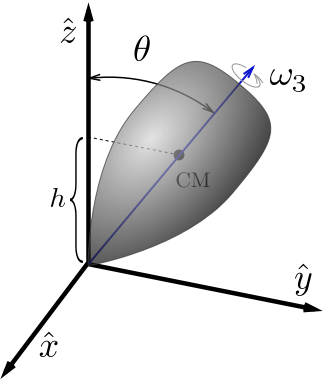
\includegraphics[width=0.3\linewidth]{./lect24/1.png}
\end{center}
Lets move from center of mass to fixed point, then
$$I^* = \begin{pmatrix}
I_1&0&0\\0&I_2&0\\0&0&I_3
\end{pmatrix}+\begin{pmatrix}
\mu a^2&0&0\\0&\mu a^2&0\\0&0&0
\end{pmatrix}$$
$$\mathcal{L} = T -V$$
$$T = T_{rot} = \frac{1}{2}I^{*}_i \Omega_i^2$$
$$V = \mu gh = \mu ga\cos \theta$$
$$\mathcal{L} = \frac{1}{2} I^*_1 \left(\dot{\theta}^2 + \dot{\varphi}^2 \sin^2 \theta\right) + \frac{1}{2} I^*_3 \left( \dot{\varphi} \cos \theta + \dot{\psi}\right)^2 - \mu g a \cos \theta$$
We can calculate momenta:
$$\begin{cases}
P_\theta = I^*_1 \dot{\theta}\\
P_\psi = I^*_2 \left(\psi\right) = L_3\\
P_\varphi = I^*_1 \dot{\varphi} sin^2 \theta + I^*_3 \left(\dot{\varphi}  \cos \theta + \dot{\psi}\right)\cos \theta = L_z
\end{cases}$$
The conserved values are canonical momenta of $\psi$ (angular momentum around $3$-axis) and $\varphi$  (angular momentum around $z$-axis)  and energy. 

$$H  = \frac{P_\theta^2}{2I^*_1} + \frac{\left(P_\varphi - P_\psi\cos \theta\right)^2}{2I^*_1 \sin^2 \theta} + \frac{P_\psi^2}{2I^*_3} +\mu ga\cos \theta$$
Define
$$U_{eff} (\theta) = \frac{\left(L_z - L_3 \cos \theta \right)^2}{2I^*_1 \sin^2 \theta} - \mu g a (1-\cos \theta ) + \left( \frac{L_3^2}{2I^*_3}  +\mu ga  \right)$$
Then
$$H(\theta, P_\theta) = \frac{P_\theta^2}{2I^*_1} + U_{eff} = E$$
$$\frac{d\theta}{dt} = \frac{\partial H}{\partial P_\theta} = \frac{P_\theta}{I^*_1} = \frac{\sqrt{2I^*_1\left(E-U_{eff}(\theta)\right)}}{I^*_1}$$
$$t  =\int \frac{I^*_1d\theta}{\sqrt{2I^*_1\left(E-U_{eff}(\theta)\right)}}$$
That allows us to find $\theta$. For $\varphi$ and $\psi$:
$$\begin{cases}
\dot{\varphi} = \frac{L_z-L_3\cos \theta}{I^*_1 \sin^2 \theta}\\
\dot{\psi} = \frac{L_3}{I^*_3}-\dot{\varphi}\cos \theta
\end{cases}$$

\begin{center}
	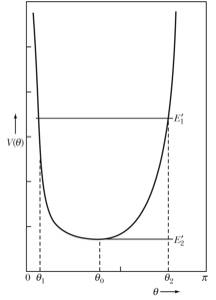
\includegraphics[width=0.3\linewidth]{./lect24/3.jpg}
\end{center}
Since effective potential goes to infinity in $\theta=0$ and $\theta=\pi$ (given $L_z\neq L_3$), the equation $E=U_{eff}$ has two solutions $\theta_1$ and $\theta_2$ and gyroscope will oscillate between them. 

If $L_z-L_3\cos \theta > 0$ for all $\theta$, $\dot{\varphi} $ doesn't change it sign and we get nutation. If its value changes sign for some $\theta$, then we get second case, in which the trajectory has loops. In the limit, if $\dot{\varphi} = 0$ exactly for $\theta_2$ (or $\theta_1$) we get third type of trajectories.

\begin{center}
	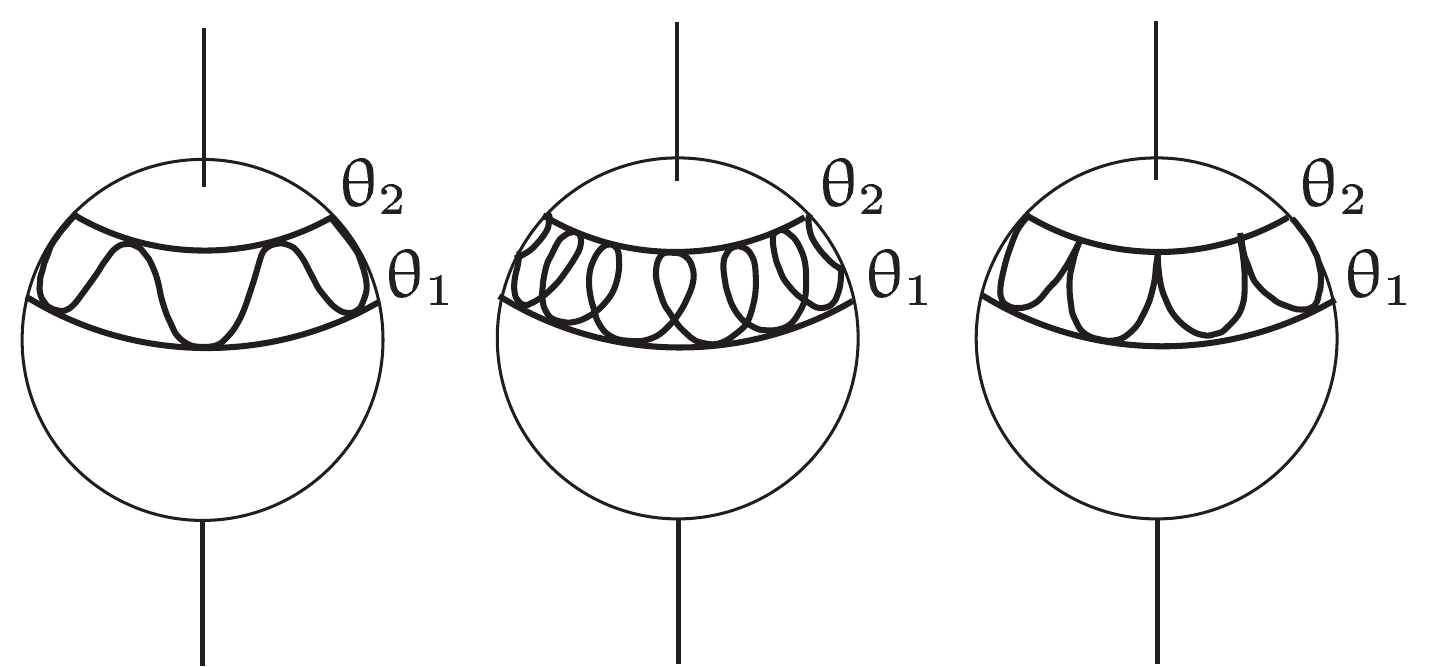
\includegraphics[width=\linewidth]{./lect24/2.png}
\end{center}
